\documentclass[11pt,a4paper]{article}
\usepackage[utf8]{inputenc}
\usepackage{graphicx}
\usepackage[load-configurations = abbreviations]{siunitx}
\usepackage[left=3cm,right=3cm,top=3cm,bottom=3cm]{geometry}
\usepackage{listings}
\usepackage{cprotect}
\usepackage{subcaption}
\title{Primo report: Studio del sistema di scintillatori}
\author{MIRACLE experiment}
\date{\today}

\begin{document}

\maketitle
\section{Introduzione}
Il seguente report riassume le misure preliminari eseguite al fine di caratterizzare, nei limiti delle nostre possibilità, il funzionamento del \textit{sistema di scintillatori}, ovvero degli scintillatori plastici che costituiscono il nostro sistema di rivelazione principale per la rivelazione della componente carica dei raggi cosmici. Le misure eseguite ad oggi sono:
\begin{itemize}
    \item Misure del rate in singola per ogni mattonella;
    \item Misure di efficienza complessiva per ogni mattonella (quindi dell'intero sistema scintillatore + SiPM) ;
    \item Misure di efficienza di alcune configurazioni di \textit{doppie}, ovvero misure sull'AND di alcune mattonelle;
    \item Misure del rate di \textit{doppie} con mattonelle montate sul frame interno, quindi nella configurazione finale per il nostro esperimento.
\end{itemize}

\section{Misure sul rate in singola}
Ricordiamo brevemente le caratteristiche di una singola mattonella. Le mattonelle di scintillatore plastico hanno dimensioni di $15\times15\times2\, \rm{cm^3}$, con una regione attiva più piccola di circa $12\times12\times2\, \rm{cm^3}$. I fotoni di scintillazione vengono convogliati nella zona dei SiPM dal rivestimento della mattonella e passando uno strato di grasso ottico + silicone speciale di protezione impattando sulla loro superficie sensibile. 
Il segnale da essi prodotto viene prima amplificato e dunque, fissando una opportuna soglia di trigger, viene discriminato in modo da poter essere \textit{contato} dei contatori della xlr8.

\subsection{Dark counts \& background}
Morsani ha eseguito dei test per verificare che i segnali in uscita dall'amplificatore siano effettivamente prodotti da un \textit{evento fisico}, ovvero un cosmico che attraversa la mattonella. Praticamente si è osservato all'oscilloscopio lo spettro in ampiezza dei segnali
con SiPM messo al buio dentro una scatolina (ovviamente staccati dallo scintillatore), figura \ref{fig:dark}. L'istogramma in rosso mostra le ampiezze, i segnali sono quelli in verde %(che sono stati acquisiti in una modalità particolare, credo persistenza?) 
e la soglia di trigger è \SI{-14.7}{mV} (edge trigger negative). Nella figura si vedono $4373$ trigger e si osserva che appaiono singoli segnali fino a quasi \SI{-60}{mV}, circa l'1 per mille supera i \SI{-30}{mV}. In conclusione, si tratta di uno spettro decrescente che si esaurisce molto rapidamente in un range facilmente escludibile settando una soglia più alta.

\begin{figure}
    \centering
    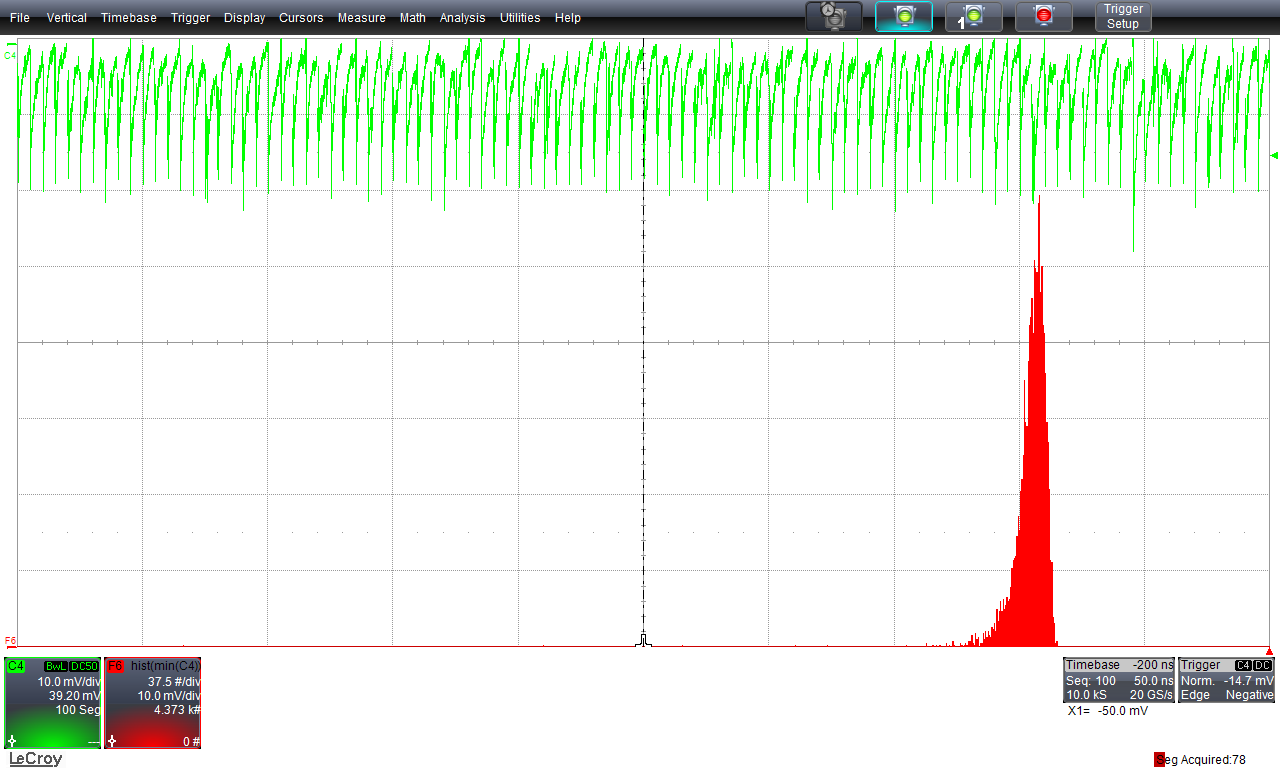
\includegraphics[scale=0.3]{Immagini/dark_counts.png}
    \caption{Istogramma dei dark counts.}
    \label{fig:dark}
\end{figure}

Lo spettro tipico che appare accoppiando il SiPM alla mattonella scintillatrice è mostrato in figura \ref{fig:signal}. Sono stati acquisiti 1700 segnali (non conosciamo l'intervallo temporale di acquisizione, quindi il numero assoluto non è molto significativo) ma ora il trigger è settato a \SI{-50}{mV} e il fondo scala è \SI{400}{mV/divisione}, contro i \SI{10}{mV/divisione} del plot \ref{fig:dark}. I trigger della Cosmocube sono impostati a circa \SI{-135}{mV} quindi siamo ragionevolmente sicuri che i dark counts rappresentano un fondo trascurabile per la nostra misura.

\begin{figure}[ht!]
    \centering
    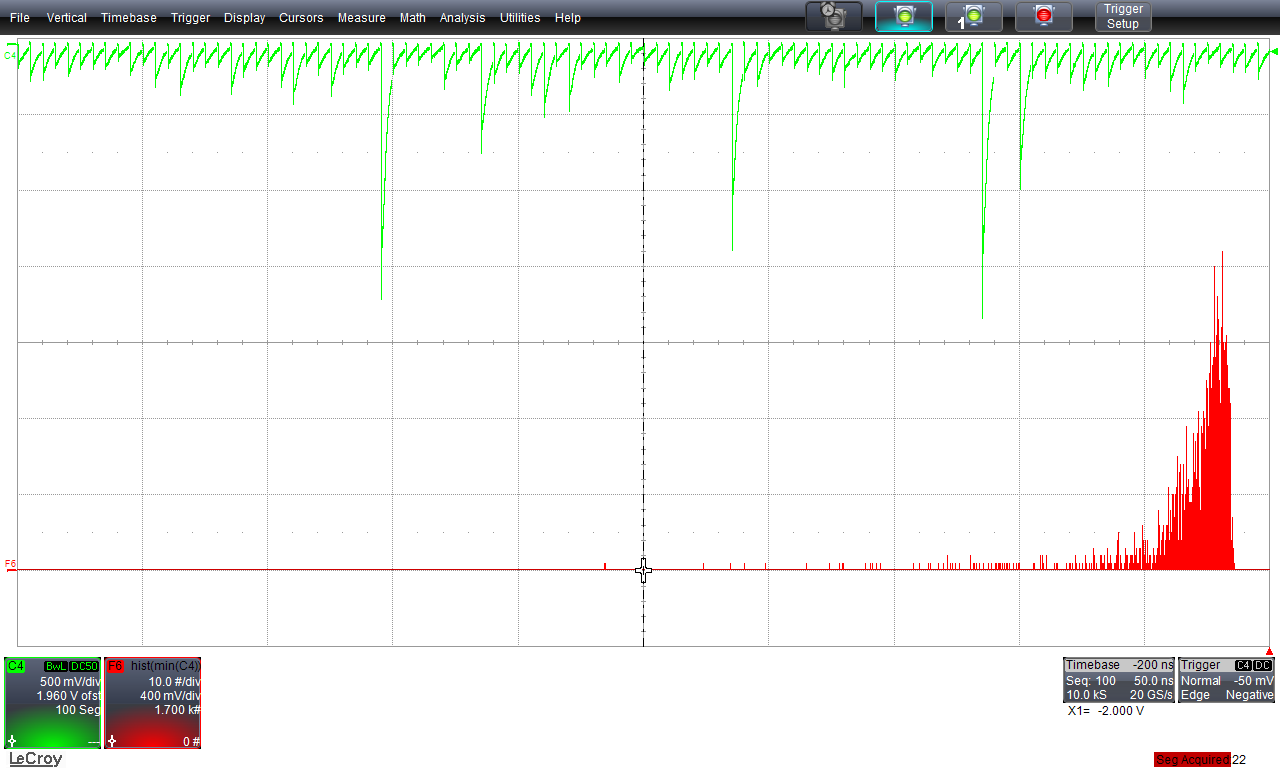
\includegraphics[scale=0.3]{Immagini/signal.png}
    \caption{Istogramma del segnale ottenuto accoppiando SiPM e scintillatore.}
    \label{fig:signal}
\end{figure}
\subsection{Conteggi in singola}
Per eseguire i conteggi di singola abbiamo disposto tutte le mattonelle in orizzontale e vicine l'una con l'altra. Oltre a caratterizzare le 3 mattonelle del telescopio abbiamo richiesto a Morsani altre 2 di \textit{riserva} e,  di queste, una rappresenta la sostituta della MM nel caso in cui quest'ultima non dovesse essere pronta a volare (piano B, come consigliato da Pilo).

L'acquisizione è durata complessivamente $T\sim \SI{2}{h}\, \SI{30}{min}$ e il numero di conteggi registrati per ogni singola mattonella è in figura \ref{fig:rate_20210921}. 

\begin{figure}[ht!]
    \centering
    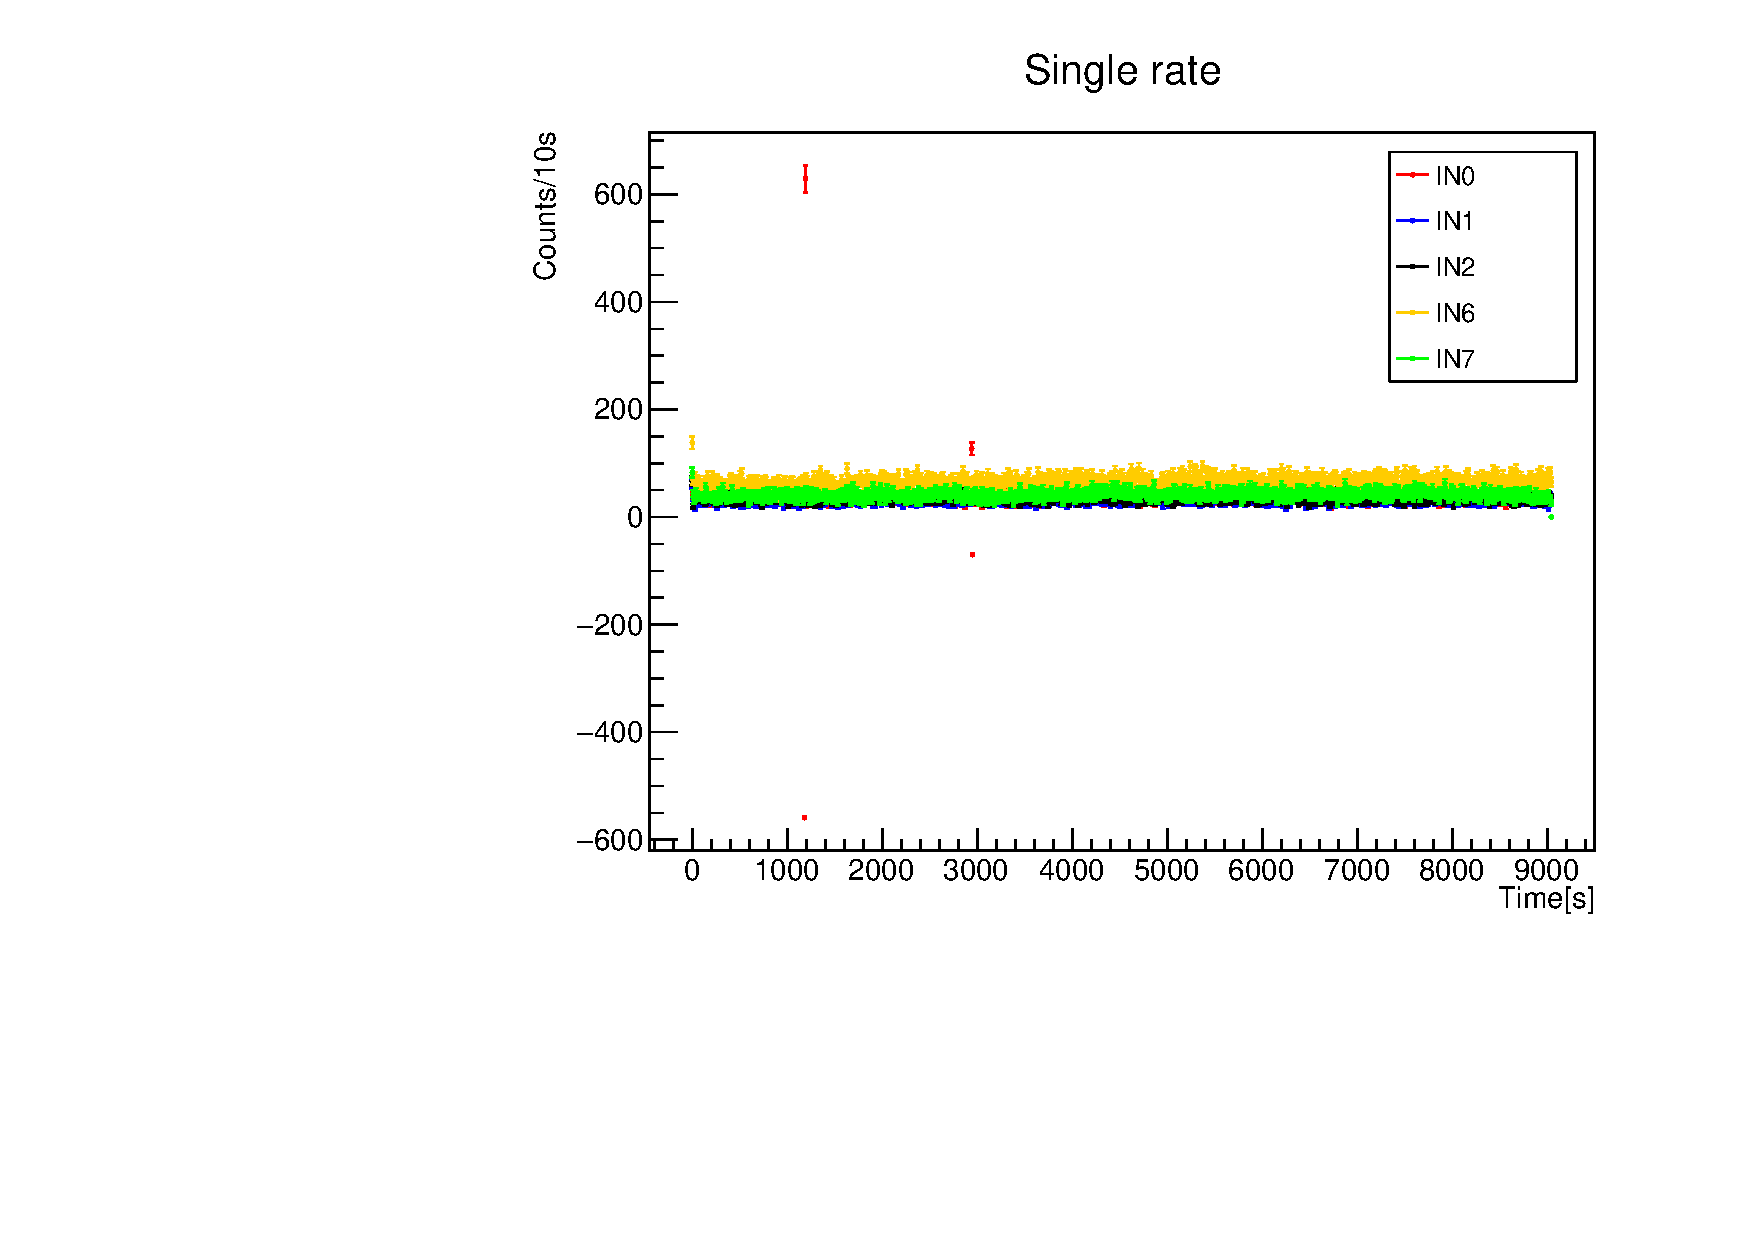
\includegraphics[scale=0.5]{Immagini/single_rate_20210921.pdf}
    \caption{Numero di eventi vs tempo di acquisizione dallo start (dati acquisiti il 21/09/2021). L'incertezza su ogni punto sperimentale è Poissoniana e i rate complessivi sono raccolti in tabella \ref{tab:rate_20210921}.}
    \label{fig:rate_20210921}
\end{figure}

In figura sono mostrati i conteggi memorizzati dai contatori della xlr8 ogni 10 secondi. Per essere precisi, i contatori della xlr8 accumulano i conteggi ogni \SI{10}{s} sommandoli a quelli registrati nell'intervallo precedente. Nel plot in figura \ref{fig:rate_20210921} ogni punto, ad un dato t ricavato dal Timestamp, viene ottenuto sottraendo al contatore il numero di conteggi precedenti all'ultimo aggiornamento. In questo modo, ogni \SI{10}{s} abbiamo effettivamente il numero di conteggi \textit{veri} degli eventi che hanno prodotto segnale nella mattonella. Inoltre, il grafico è stato ottenuto con il codice di analisi, \verb|analysis.C|, scritto in C/C++ ed eseguito con il software ROOT che prende in input il file:
\begin{verbatim}
        20210921_data_xlr8.log
\end{verbatim}
comunque si rimanda allo script per eventuali chiarimenti sulle procedure.
Può essere interessante soffermarsi sugli outliers che si presentano per IN0. Questi punti sono una conseguenza di conteggi anomali memorizzati dalla xlr8 che non sono contenuti nell'intervallo definito dal conteggio precedente e da quello successivo. Per esempio se guardiamo nel file di dati il punto a circa \SI{1200}{s} abbiamo 3327 conteggi che non appartiene all'intervallo [3886,3956], tabella \ref{tab:outlier}. Quindi il punto si ottiene calcolando $3956-3327=629$ è un outlier, ma anche $3327-3886=-559$ è outlier e in questo modo si spiega anche perché ci sono valori negativi. La natura fisica di questo problema potrebbe essere una lettura del contatore in \textit{simultanea} alla transizione dei bit del contatore stesso, ma stiamo ancora ragionando sulla causa.
\begin{table}
    \centering
    
\end{table}

Comunque i rate ottenuti per le singole mattonelle, calcolati prendendo l'ultimo conteggio dei registi prima di arrestare l'acquisizione diviso il tempo totale di presa dati è riportato in tabella \ref{tab:rate_20210921}.


\begin{table}
\begin{subtable}[c]{0.6\textwidth}
\centering
\begin{tabular}{ccc}
    \hline
    Timestamp[s] & Reset time [s] & IN0 \\
    \hline
    \hline
    ... & ... & ...\\
    1521109323.095752 & 1162 & 3886 \\
    1521109333.078572 & 1172 & \textbf{3327} \\
    1521109343.090377 & 1182 & 3956 \\
    ... & ... & ...\\
    \hline
    \end{tabular}
    \subcaption{Estratto dal file di dati righe 120-122.}
    \label{tab:outlier}
\end{subtable}
\begin{subtable}[c]{0.4\textwidth}
\centering
\begin{tabular}{cc}
    \hline
    & Rate [Hz] \\
    \hline
    \hline
    IN0 & $\sim 3.4$ \\
    IN1 & $\sim 3.1$ \\
    IN2 & $\sim 3.5$ \\
    IN6 & $\sim 6.6$ \\
    IN7 & $\sim 4.1$ \\
    \hline
    \end{tabular}
    \subcaption{Rate singole.}
    \label{tab:rate_20210921}
\end{subtable}
\end{table}
In virtù dei risultati ottenuti, abbiamo deciso di escludere la mattonella $\#6$ e di usare la mattonella $\#7$ come \textit{riserva}; mentre le altre tre mattonelle costituiranno il sistema di rivelazione principale del telescopio.
\subsection{Misure di efficienza}
\subsection{Stabilit\'a temporale dei conteggi}
Successivamente alle misure di efficienza, nel periodo tra il 21/09 e il 7/10 sono state effettuate delle prese dati lunghe, in modo da studiare la stabilità temporale dei conteggi in singola e in doppia. In questo studio è stata esclusa lo scintillatore $\#6$ per i motivi di cui sopra. Di seguito sono i riportati i plot delle prese dati. \textbf{N.B}. : i plot sono riportati senza gli errori sui conteggi e con binning differenti, per permettere una lettura più semplice. I conteggi in doppia sono realizzati come :
\begin{itemize}
\item[AND0] : $\#0$ AND $\#7$ (flusso verticale);
\item[AND1] : $\#1$ AND $\#7$ (flusso orizzontale);
\item[AND2] : $\#0$ AND $\#1$ (flusso obliquo);
\end{itemize}
\begin{figure}
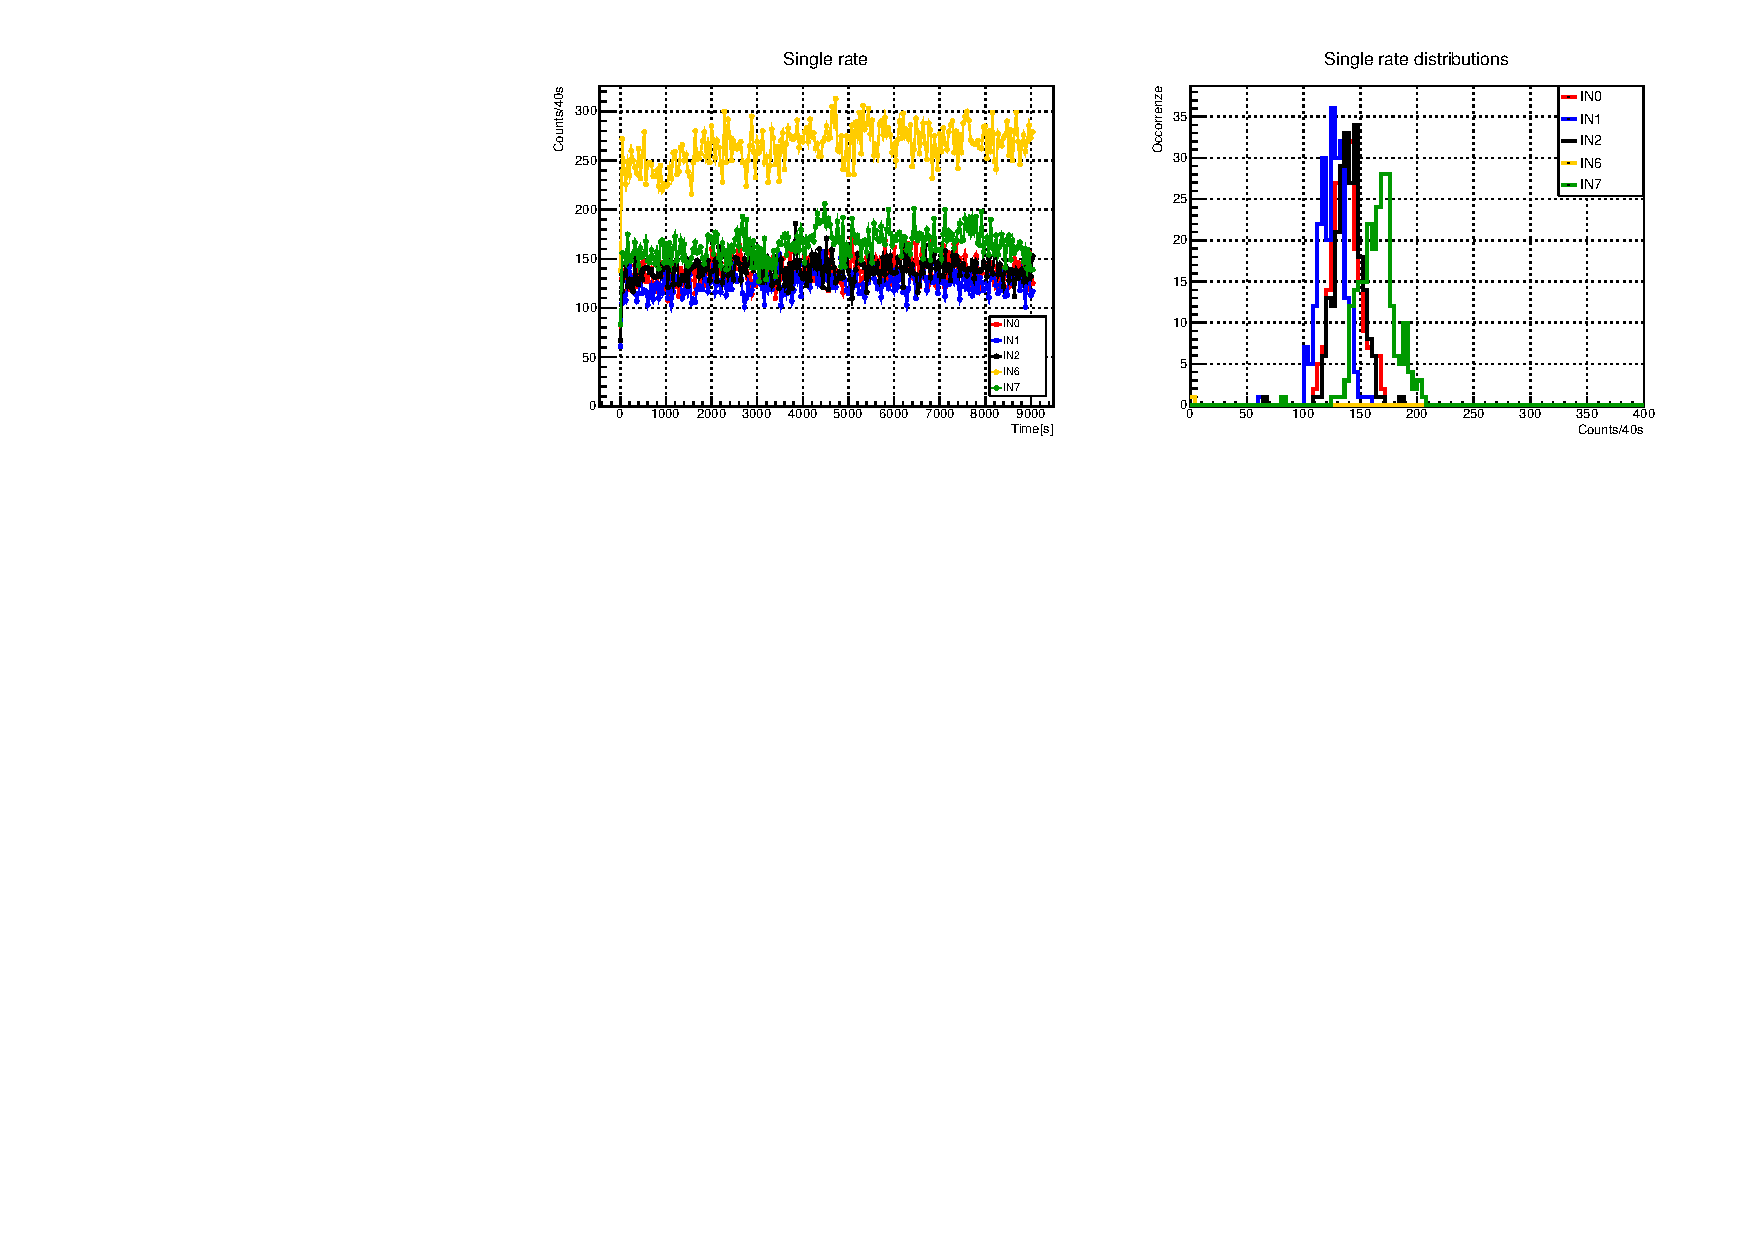
\includegraphics[width=0.9\textwidth]{Immagini/20210921.pdf}
\caption{Presa dati del 21-09-2021.}
\end{figure}  
\begin{figure}
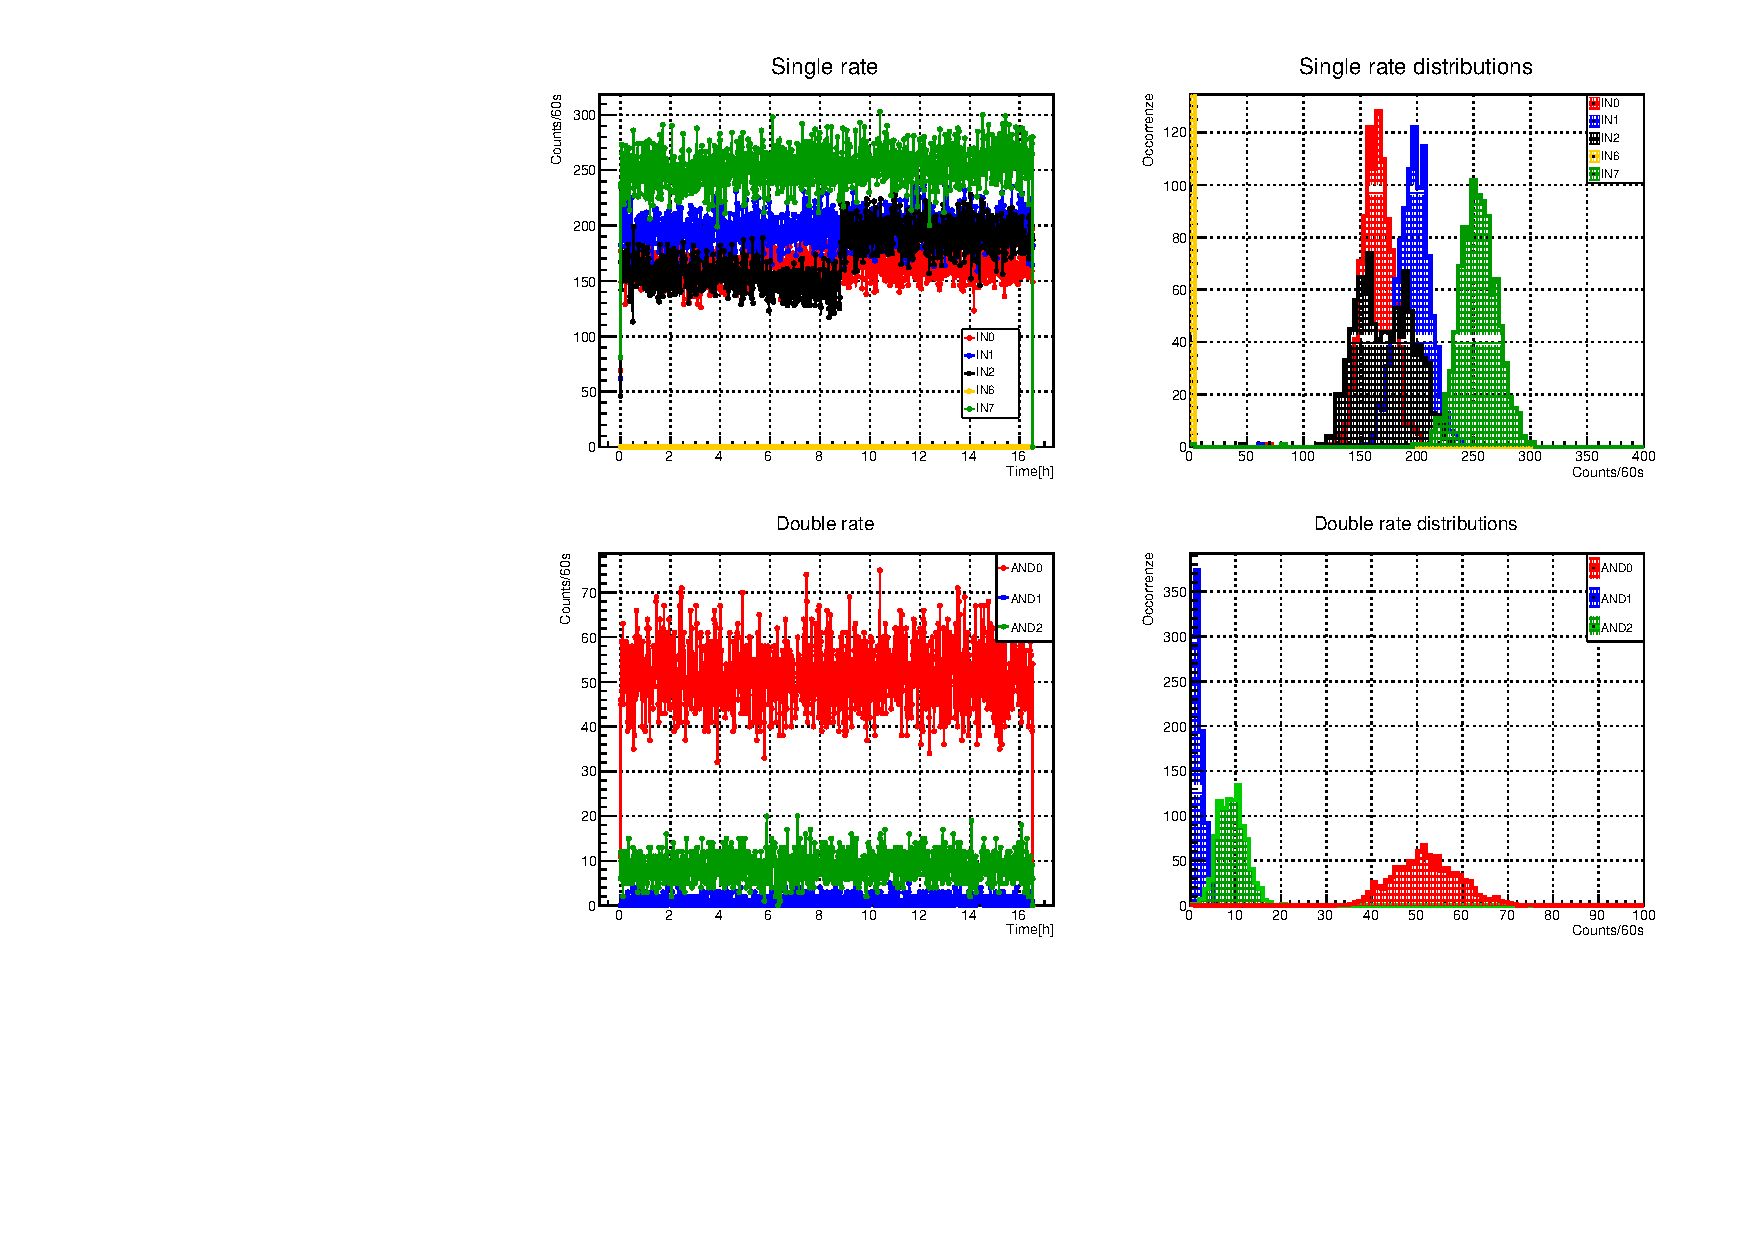
\includegraphics[width=0.9\textwidth]{Immagini/20210928.pdf}
\caption{Presa dati del 28-09-2021.}
\end{figure}  \begin{figure}
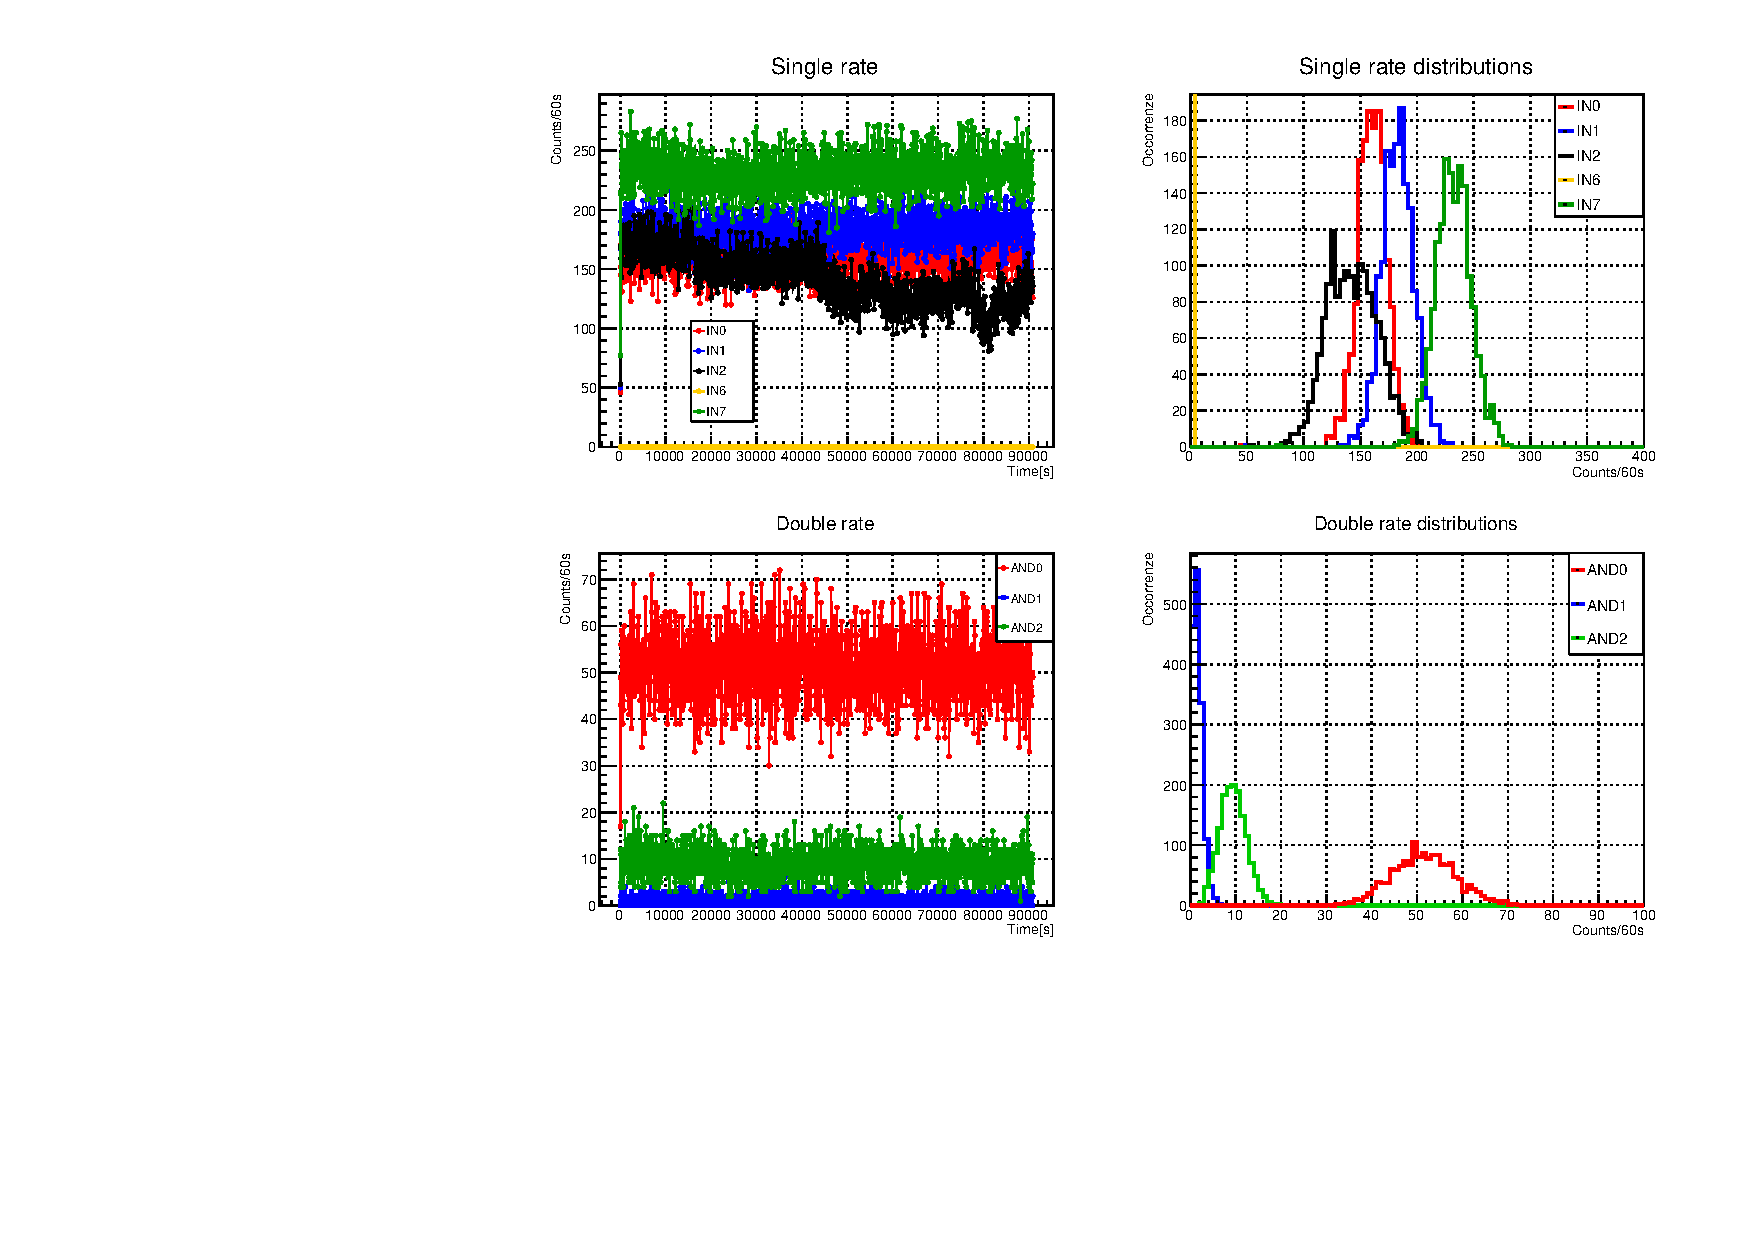
\includegraphics[width=0.9\textwidth]{Immagini/20210930.pdf}
\caption{Presa dati del 30-09-2021.}
\end{figure}  \begin{figure}
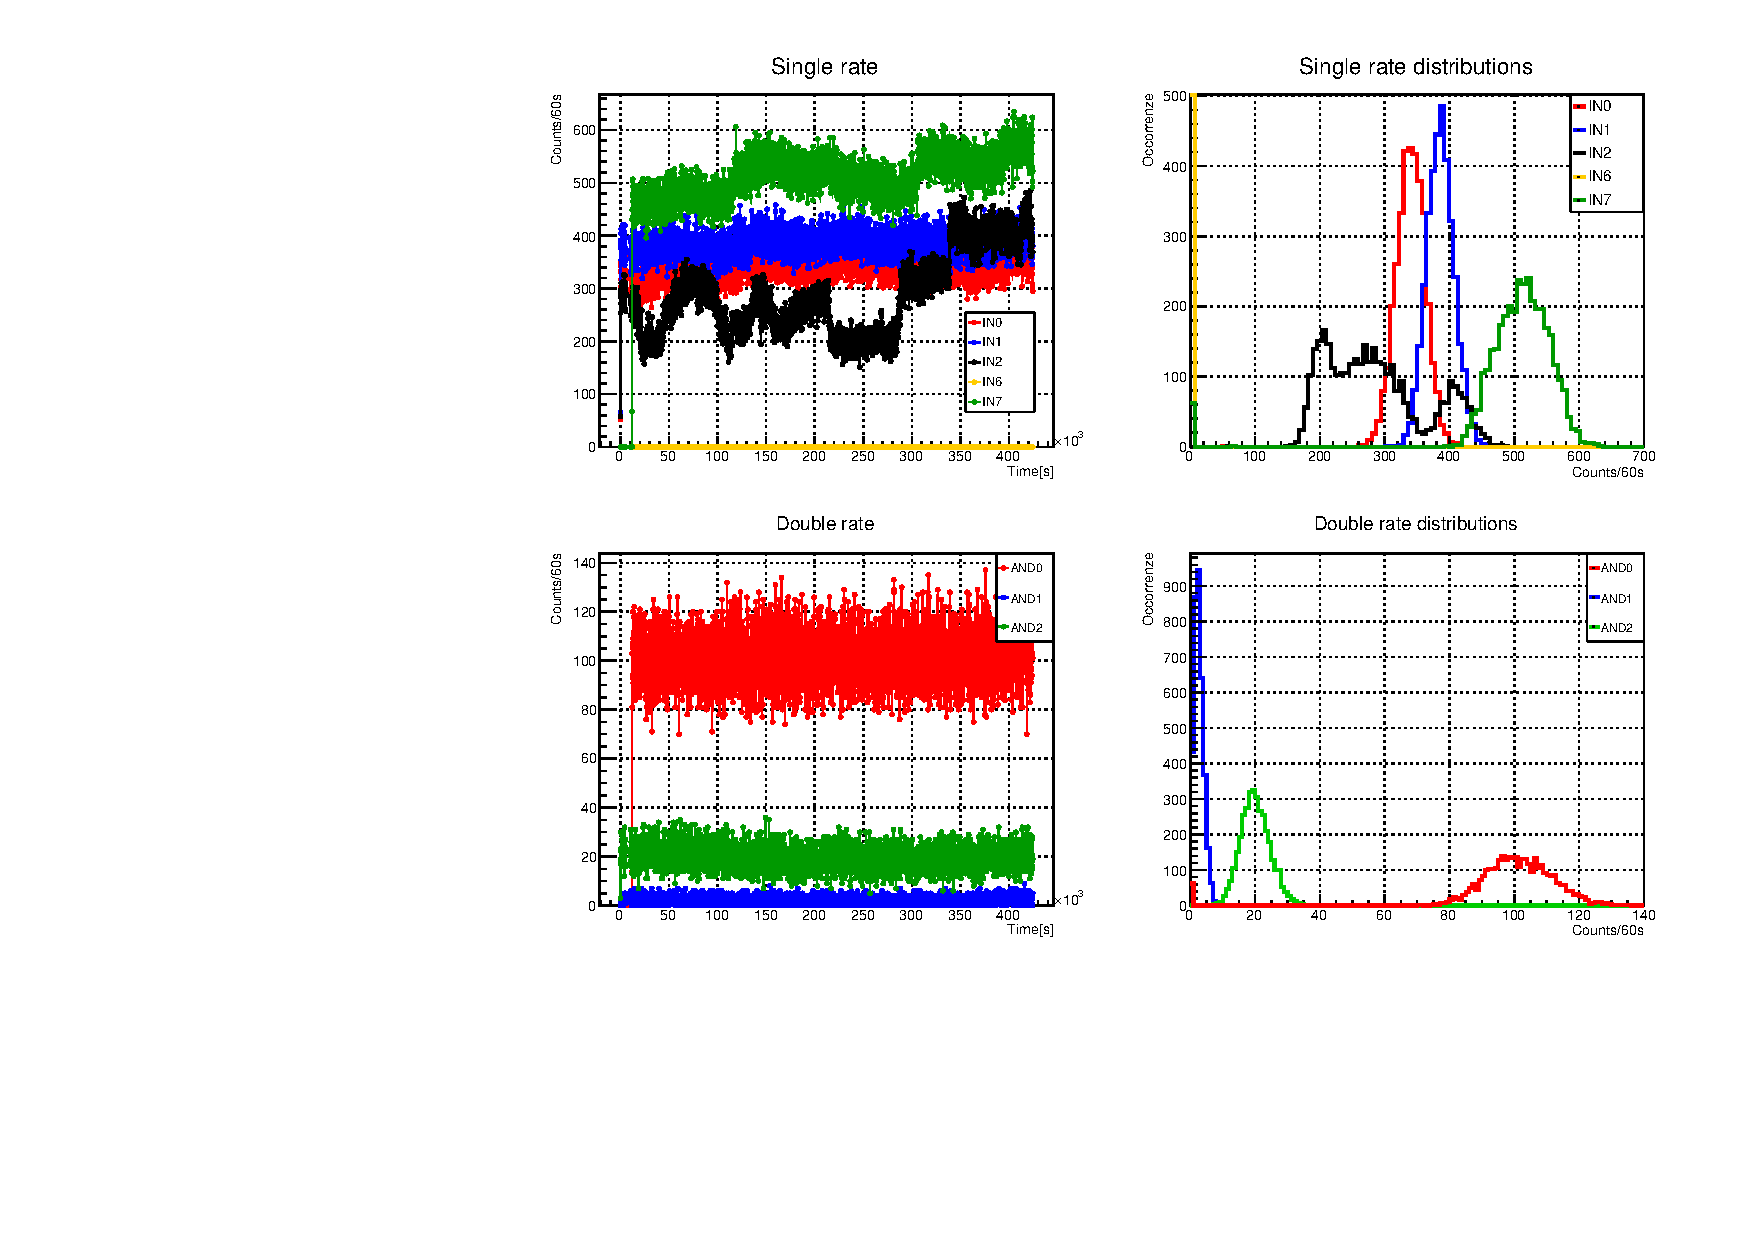
\includegraphics[width=0.9\textwidth]{Immagini/20211005.pdf}
\caption{Presa dati del 05-10-2021.}
\end{figure} \begin{figure}
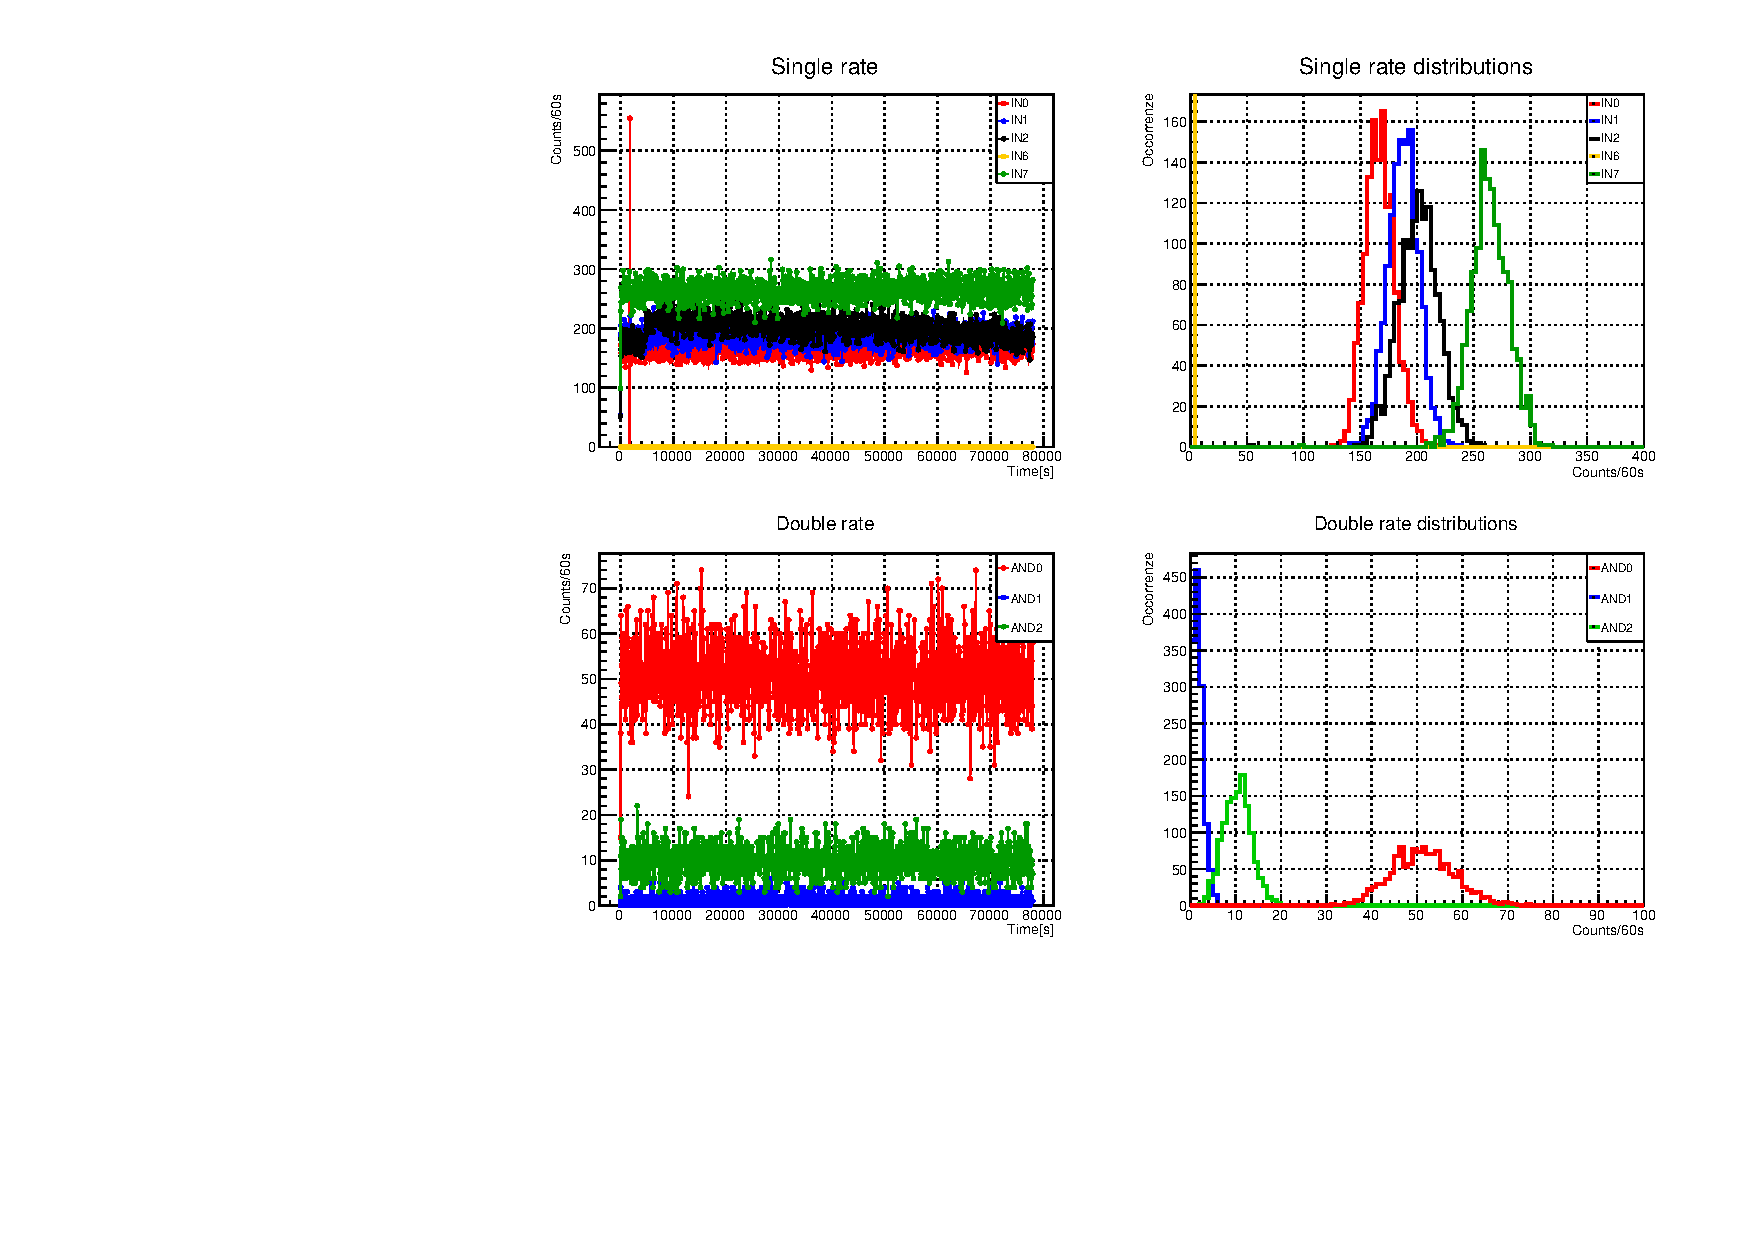
\includegraphics[width=0.9\textwidth]{Immagini/20211006.pdf}
\caption{Presa dati del 06-10-2021.}
\end{figure}   
\end{document}

